\documentclass[pdf, aspectratio=169]{beamer}
\usepackage[]{hyperref, graphicx, siunitx, lmodern, tikz, booktabs, physics,tensor}
\usepackage[mode=buildnew]{standalone}
\usepackage{pdfpc-commands}
\usepackage{intro-commands}

\usetheme{Astro}
\graphicspath{ {../Images/} }

\sisetup{per-mode=symbol}
\usetikzlibrary{calc, patterns, decorations.markings, decorations.pathmorphing, shapes}
\tikzstyle{proton}=[circle, minimum size = 7mm, ball color=red, black,transform shape]
\tikzstyle{neutron}=[circle, minimum size=7mm, ball color=gray, black, transform shape]
\tikzstyle{gammaray}=[ultra thick, -latex, decorate, decoration={snake, post length=3mm}]

%Preamble
\title{A Mass of Incandescent Gas}
\author{Jed Rembold}
\date{October 24, 2018}

\begin{document}
\renewcommand{\theenumi}{\Alph{enumi}}

\begin{frame}{Announcements}
	\begin{itemize}
		\item Nothing due on Friday
		\item Test 2 on Friday!!
			\begin{itemize}
				\item Solar System material (Ch7-14)
				\item All review materials posted (with solutions)
				\item Equation page updated
				\item Email me if you want to reserve one of my few calculators for Friday 			\end{itemize}
		\item Polling: \nolinkurl{rembold-class.ddns.net}
	\end{itemize}
\end{frame}

%\begin{frame}{Astronomy Picture of the Day}
  %\begin{center}
	%\includegraphics[width=.75\textwidth]{APOD_MoonHole.jpg}
  %\end{center}
%\end{frame}

\begin{frame}{Review Question!}
  Our Sun is powered by:
  \begin{enumerate}
	\item \alert<2>{Fusion}
	\item Fission
	\item Gravitational Collapse
	\item Solar Power
  \end{enumerate}
\end{frame}

\begin{frame}{Fusion Power!}
  \begin{itemize}
	\item The interior of the Sun is very dense, very hot, and very Hydrogen
	\item Packs lots of protons close together and moving real fast
	\item When protons get close enough:
	  \begin{itemize}
		\item Bang! Fusion happens!
		\item Energy is given off!
		\item The cycle continues\ldots
	  \end{itemize}
  \end{itemize}
\end{frame}

\begin{frame}{The Sun is a Mass\ldots}
  \begin{center}
	\inlineMovie{../Videos/SunIsAMass.ogv}{../Videos/SunIsAMass.png}{width=.45\textwidth}
	\url{https://www.youtube.com/watch?v=me06I9GDM_k}
  \end{center}
\end{frame}

\begin{frame}{Fusion vs Fission: The Periodic Table}
  \begin{center}
	\begin{tikzpicture}[scale=.85, transform shape]
	  \node[inner sep=0pt, outer sep=0pt, anchor=south west] at (0,0) {\includegraphics[width=\textwidth]{ch11_periodictable.png}};
	  %\draw[help lines] (0,0) grid (12,7);
	  \fill<2>[cyan, opacity=0.4] (2.0,6.7) --++(10,0) --++(0,-1.85) --++(-6.1,0) --++(0,-.6) --++(-3.9,0);
	  \node<2>[white, font=\LARGE] at (4.5,5.5) {Fusion};
	  %\fill<3>[orange, opacity=0.4] (1.6,3.26) -- (5,3.26) -- (5,3.75) -- (9.1,3.75) -- (9.1,0.6) -- (1.6,0.6);
	  \fill<3>[orange, opacity=0.4] (6.45,4.85)--+(5.5,0) --+(5.5,-4.2) --+(-4.5,-4.2) --+(-4.5,-.6)--++(0,-.6);
	  \node<3>[white, font=\LARGE] at (10,2.5) {Fission};
	\end{tikzpicture}
  \end{center}
\end{frame}

\begin{frame}{Powering Your Sun: A 3 Step Process}
  \begin{center}
	\begin{tikzpicture}
	  \onslide<1->{
		\coordinate (col1) at (1,0);
		\draw[ultra thick, cyan, -latex] (0,2) node[proton] {p} -- (col1);
		\draw[ultra thick, cyan, -latex] (0,-2) node[proton] {p} -- (col1);
		\draw[ultra thick, orange, -latex] (col1) --+(60:1.5) node[right] {$e^+$};
		\node[proton] (p1) at ($(col1)+(2,0)$) {p};
		\node[neutron] (n1) at ($(p1)+(4mm,0)$) {n};
		\draw[ultra thick, orange, -latex] (col1) --(p1);
		\draw[ultra thick, orange, -latex] (col1) --+(-60:1.5) node[right] {$\nu$};
	  }
	  \onslide<2->{
		\draw[ultra thick, cyan, latex-] (n1) --+(-100:2) node[proton] {p};
		\node[proton](p2) at ($(n1)+(2,0)$) {p};
		\node[proton] at ($(p2)-(0,4mm)$) {p};
		\node[neutron](n2) at ($(p2)+(-30:4mm)$) {n};
		\draw[orange, ultra thick, -latex] (n1) -- (p2);
		\draw[orange, gammaray] (n1) --+(60:2) node[right] {$\gamma$};
		\fill[Background, opacity=0.6] (-1,-3) rectangle (2.6,3);
	  }
	  \onslide<3->{
		\node[proton](p3) at ($(p2)+(0,-2)$) {p};
		\node[proton] at ($(p3)-(0,4mm)$) {p};
		\node[neutron](n3) at ($(p3)+(-30:4mm)$) {n};
		\draw[ultra thick, cyan, -latex] (p3) -- (n2);
		\draw[ultra thick, orange, -latex] (n2) --+(60:2) node[anchor=south west,proton] {p};
		\draw[ultra thick, orange, -latex] (n2) --+(-60:2) node[anchor=north west,proton] {p};
		\draw[ultra thick, orange, -latex] (n2) --+(2,0) node[anchor=west, proton] (p4) {p};
		\node[neutron] at ($(p4)+(60:4mm)$) {n};
		\node[proton] at ($(p4)+(0:6mm)$) {p};
		\node[neutron] at ($(p4)+(-60:4mm)$) {n};
		\fill[Background, opacity=0.6] (-1,-3) rectangle (5,3);
	  }
	\end{tikzpicture}
	\onslide<3->{\[4\left( \nuclide[1][1]{H} \right) \rightarrow \nuclide[4][2]{He} + 2e^+ + 2\nu + \gamma\]}
  \end{center}
\end{frame}

\begin{frame}{Taking things slow\ldots}
  \begin{itemize}
	\item The full 3 step reaction is actually quite slow!
	\item First Step:
	  \begin{itemize}
		\item The tricky one
		\item Need both to get \alert{really} close AND need the proton to decay into a neutron
		\item Takes over a billion years!
	  \end{itemize}
	\item Second Step:
	  \begin{itemize}
		\item Quite fast
		\item About 1 second
	  \end{itemize}
	\item Third Step:
	  \begin{itemize}
		\item Slow again, but 1000$\times$ faster than Step 1
		\item About a million years
	  \end{itemize}
	\item The sheer number of protons is what maintains such a high energy output!
  \end{itemize}
\end{frame}

\begin{frame}{The Photon Trail\ldots}
  \begin{itemize}
	\item Our mechanism for fusion releases much of the energy in gamma rays
	\item But Gamma Rays are not the majority of what we see coming out of the Sun! (Thankfully!)
	\item Something else must be happening enroute
	  \begin{itemize}
		\item Not much between us and the Sun, so most likely in the Sun itself
	  \end{itemize}
  \end{itemize}
  \begin{center}
	\includegraphics[width=.8\textwidth]{ch11_hulk.jpg}
  \end{center}
\end{frame}

\begin{frame}{\ldots a crooked path}
  \begin{columns}
	\column{.5\textwidth}
	\begin{itemize}
	  \item Gas below photosphere is very dense and ionized
		\begin{itemize}
		  \item Photons interact with charged particles
		  \item ``Scattered'' by nuclei and electrons
		  \item Results in a ``random walk'' to the surface
		\end{itemize}
	  \item Energy produced in the core thus takes many thousands of years to reach the surface
	  \item The photons we see on Earth tell us about the \emph{photosphere}
	  \item We do \emph{not} get to see into the core
	\end{itemize}
	\column{.5\textwidth}
	\begin{center}
	  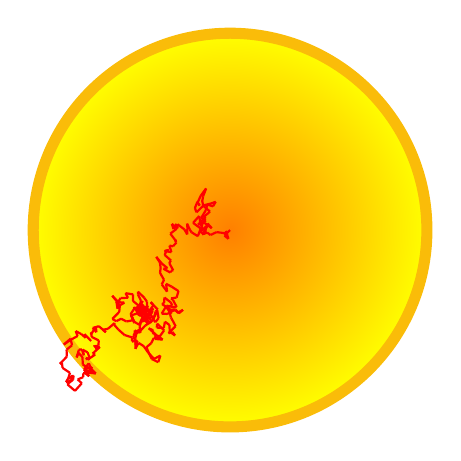
\begin{tikzpicture}
		\draw[yellow!50!orange, line width=4pt, inner color = orange, outer color=yellow] (0,0) circle (2.5cm);
		\coordinate (old) at (0,0);
		\foreach \t in {1,2,...,350}{
		  \draw[red, thick] (old) --+ (rand/10,rand/10) coordinate (old);
		}
	  \end{tikzpicture}
	\end{center}
  \end{columns}
\end{frame}

\begin{frame}{Nature's Atomic Hermits}
  \begin{columns}
	\column{.5\textwidth}
	\begin{center}
	  \vspace{-8mm}
	  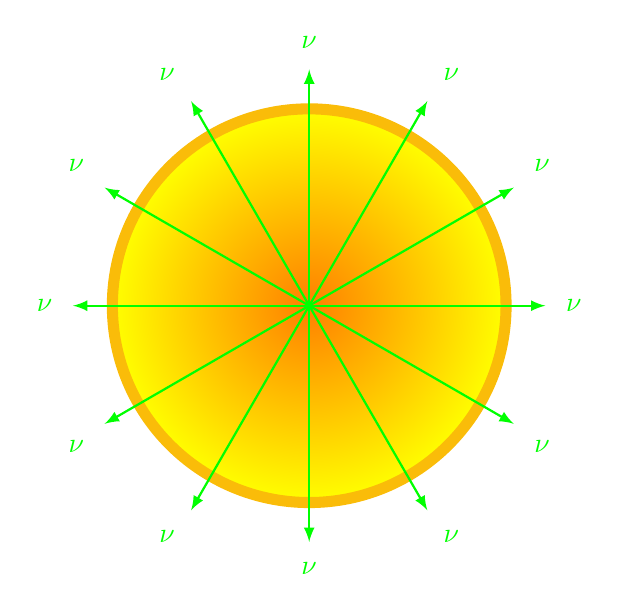
\begin{tikzpicture}
		\draw[yellow!50!orange, line width=4pt, inner color = orange, outer color=yellow] (0,0) circle (2.5cm);
		\foreach \a in {30,60,90,...,360}{
		  \draw[green, -latex, thick] (0,0) --+(\a:3) node[label={\a:$\nu$}] {};
		}		
	  \end{tikzpicture}
	\end{center}
	\column{.5\textwidth}
	\begin{itemize}
	  \item Neutrinos are notoriously inactive
		\begin{itemize}
		  \item They generally don't interact with anything
		\end{itemize}
	  \item This makes them very tricky to detect
	  \item But they COULD show us the core of the Sun!
	\end{itemize}
  \end{columns}
\end{frame}

\begin{frame}{Catch a Neutrino by its tail\ldots}
  \begin{itemize}
	\item Find an isolated area
	  \begin{itemize}
		\item Generally underground, away from other radiation
	  \end{itemize}
	\item Build a BIG detector
	  \begin{itemize}
		\item A neutrino interacting is a rare event, the bigger the detector, the better your chances
	  \end{itemize}
	\item Variety of detection methods
	  \begin{itemize}
		\item Checking huge vats of chlorine for traces of argon caused by a neutrino interaction
		\item Looking for traces of light from Cherenkov radiation, when a charged particle travels fast than light \emph{in that medium}, usually water or ice (Antarctica)
	  \end{itemize}
  \end{itemize}
\end{frame}

\fullFrameImageZoomedHorizontal{ch11_neutrino_detector_japan.jpg}

\begin{frame}{Can't Change Your Spots \scriptsize(But the Sun can!)}
  \begin{columns}
	\column{.5\textwidth}
	\begin{itemize}
	  \item Sunspots are dark patches on the surface of the photosphere
	  \item Darker because they are cooler ($\approx \SI{4000}{\kelvin}$)
	  \item Something must keep the cool gas from mixing with the surrounding hotter gas!
	\end{itemize}
	\column{.5\textwidth}
	\begin{center}
	  \includegraphics[width=.9\textwidth]{ch11_sunspots.png}
	\end{center}
  \end{columns}
\end{frame}

\fullFrameImage{ch11_sun_now.png}

\begin{frame}{The Sun's Magnetic Fields}
  \begin{columns}
	\column{.5\textwidth}
	\begin{itemize}
	  \item Sunspots give us a way to see parts of the Sun's magnetic field!
	  \item Often come in pairs, one for each magnetic pole
	  \item Seem to be loops where the magnetic field can connect
	\end{itemize}
	\column{.5\textwidth}
	\begin{center}
	  \begin{tikzpicture}
		\node[inner sep=0pt, outer sep=0pt] at (0,0) {\includegraphics[width=6cm]{ch11_sun_now_xray.jpg}};
		\node<1>[opacity = 0.0, inner sep=0pt, outer sep=0pt] at (0,0) {\includegraphics[width=4.7cm]{ch11_sun_now_vis.jpg}};
		\node<2>[opacity = 0.5, inner sep=0pt, outer sep=0pt] at (0,0) {\includegraphics[width=4.7cm]{ch11_sun_now_vis.jpg}};
		\node<3>[opacity = 1, inner sep=0pt, outer sep=0pt] at (0,0) {\includegraphics[width=4.7cm]{ch11_sun_now_vis.jpg}};
	  \end{tikzpicture}
	\end{center}
  \end{columns}
\end{frame}

\fullFrameMovie{../Videos/sdo-vid.ogv}{../Videos/sdo-vid.png}

\begin{frame}{Flareon}
  \begin{itemize}
	\item Most flares occur near sunspots, implying a connection to the magnetic field
	\item Unlike the Earth, the equator of the Sun rotates faster than the poles!
	  \begin{itemize}
		\item Think tradewinds on Earth, but the entire Sun is a gas
	  \end{itemize}
	\item Gases tend to drag the magnetic field with them
	\item Things can get very tangled, and flares are though to be a way of rearranging magnetic field lines to untangle them
  \end{itemize}
  \begin{center}
	\inlineMovie{../Videos/Flare.ogv}{../Videos/Flare.png}{width=.5\textwidth}
  \end{center}
\end{frame}

\begin{frame}{Effects on Earth}
  \begin{itemize}
	\item Communications
	\item Aurora
  \end{itemize}
  \begin{center}
	\includegraphics[height=4cm]{ch11_aurora_ground.jpg}
	\includegraphics[height=4cm]{ch11_aurora_space.jpg}
  \end{center}
\end{frame}

\fullFrameImage{ch11_solar_cycle.jpg}







\end{document}

